% PRISMA 2020 flow diagram (final, 2026-10-12). Numbers: screening/prisma_counts.md, fulltext/fulltext_decisions.csv
\documentclass[border=4pt]{standalone}
\usepackage[T1]{fontenc}
\usepackage[scaled]{helvet}
\renewcommand{\familydefault}{\sfdefault}
\usepackage{tikz}
\usetikzlibrary{positioning,arrows.meta,calc,backgrounds}
\definecolor{flow}{HTML}{DCEAF7}
\definecolor{flowline}{HTML}{0072B2}
\definecolor{excl}{HTML}{F6F6F6}
\definecolor{exclline}{HTML}{8C8C8C}
\definecolor{incl}{HTML}{FBE3D6}
\definecolor{inclline}{HTML}{D55E00}
\definecolor{band}{HTML}{0B3C5D}
\begin{document}
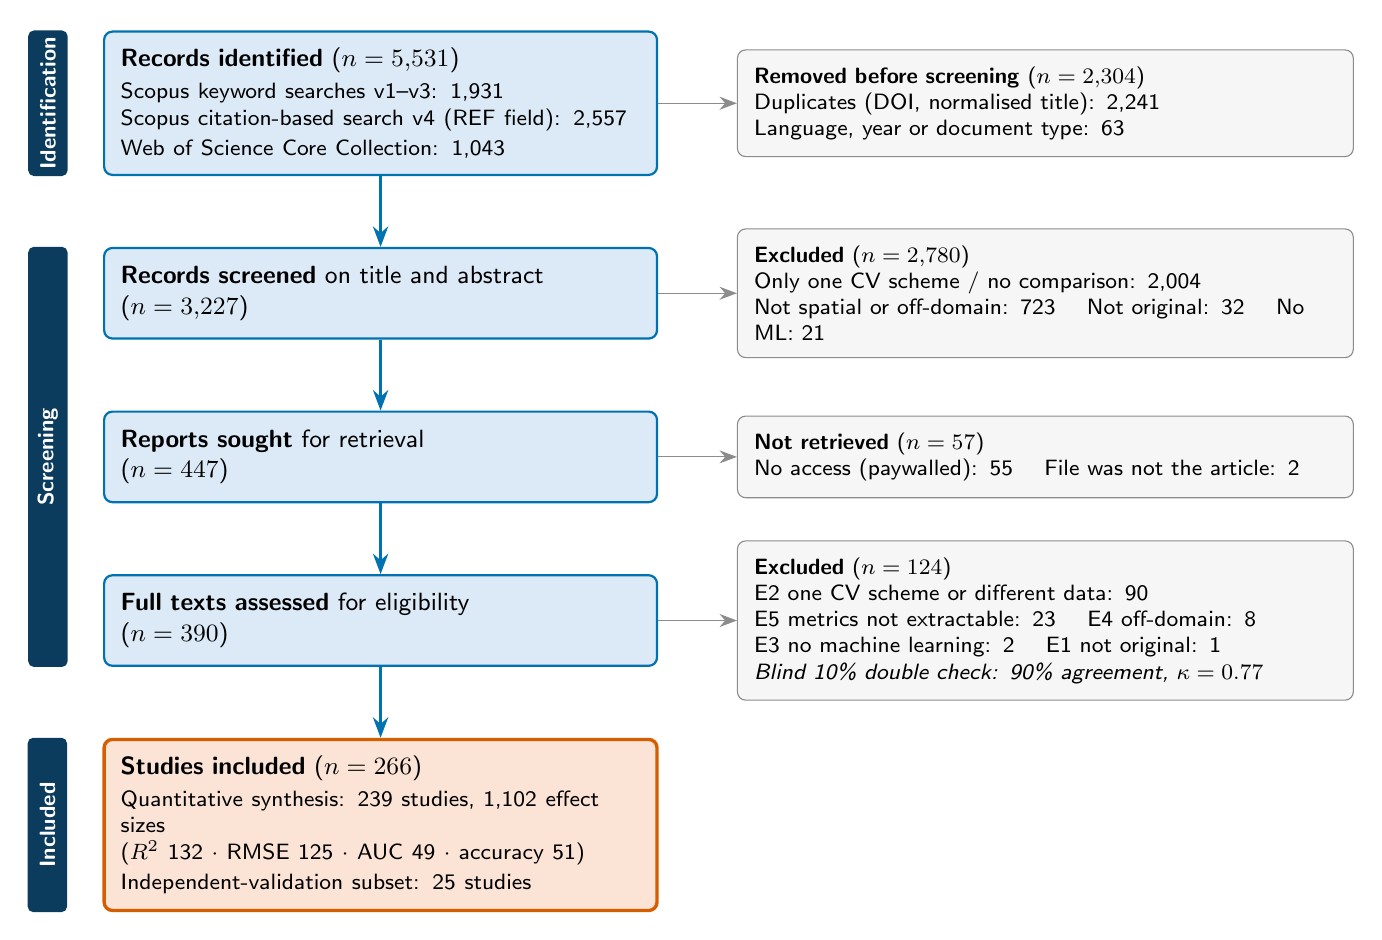
\begin{tikzpicture}[
  font=\small,
  box/.style={draw=flowline, fill=flow, rounded corners=3pt, thick, align=left, text width=6.6cm, inner sep=6pt, minimum height=1.15cm},
  side/.style={draw=exclline, fill=excl, rounded corners=3pt, align=left, text width=7.4cm, inner sep=6pt, font=\footnotesize},
  fin/.style={draw=inclline, fill=incl, rounded corners=3pt, very thick, align=left, text width=6.6cm, inner sep=6pt},
  arr/.style={-{Stealth[length=2.6mm]}, thick, draw=flowline},
  sarr/.style={-{Stealth[length=2.2mm]}, draw=exclline}]

\node[box] (id) {\textbf{Records identified} ($n = 5{,}531$)\\[2pt]
  {\footnotesize Scopus keyword searches v1--v3: 1{,}931\\
  Scopus citation-based search v4 (REF field): 2{,}557\\
  Web of Science Core Collection: 1{,}043}};
\node[side, right=1.0cm of id] (rm) {\textbf{Removed before screening} ($n = 2{,}304$)\\
  Duplicates (DOI, normalised title): 2{,}241\\
  Language, year or document type: 63};

\node[box, below=0.9cm of id] (sc) {\textbf{Records screened} on title and abstract\\ ($n = 3{,}227$)};
\node[side, right=1.0cm of sc] (ex1) {\textbf{Excluded} ($n = 2{,}780$)\\
  Only one CV scheme / no comparison: 2{,}004\\
  Not spatial or off-domain: 723 \quad Not original: 32 \quad No ML: 21};

\node[box, below=0.9cm of sc] (sought) {\textbf{Reports sought} for retrieval\\ ($n = 447$)};
\node[side, right=1.0cm of sought] (nr) {\textbf{Not retrieved} ($n = 57$)\\
  No access (paywalled): 55 \quad File was not the article: 2};

\node[box, below=0.9cm of sought] (el) {\textbf{Full texts assessed} for eligibility\\ ($n = 390$)};
\node[side, right=1.0cm of el] (ex2) {\textbf{Excluded} ($n = 124$)\\
  E2 one CV scheme or different data: 90\\
  E5 metrics not extractable: 23 \quad E4 off-domain: 8\\
  E3 no machine learning: 2 \quad E1 not original: 1\\
  \textit{Blind 10\% double check: 90\% agreement, $\kappa = 0.77$}};

\node[fin, below=0.9cm of el] (inc) {\textbf{Studies included} ($n = 266$)\\[2pt]
  {\footnotesize Quantitative synthesis: 239 studies, 1{,}102 effect sizes\\
  ($R^2$ 132 $\cdot$ RMSE 125 $\cdot$ AUC 49 $\cdot$ accuracy 51)\\
  Independent-validation subset: 25 studies}};

\draw[arr] (id) -- (sc);  \draw[sarr] (id) -- (rm);
\draw[arr] (sc) -- (sought); \draw[sarr] (sc) -- (ex1);
\draw[arr] (sought) -- (el); \draw[sarr] (sought) -- (nr);
\draw[arr] (el) -- (inc); \draw[sarr] (el) -- (ex2);

\begin{scope}[on background layer]
\foreach \top/\bot/\lab in {id/id/Identification, sc/el/Screening, inc/inc/Included}{
  \fill[band, rounded corners=2pt] ([xshift=-0.95cm]\top.north west) rectangle ([xshift=-0.45cm]\bot.south west);
  \node[rotate=90, text=white, font=\footnotesize\bfseries] at ($([xshift=-0.7cm]\top.north west)!0.5!([xshift=-0.7cm]\bot.south west)$) {\lab};}
\end{scope}
\end{tikzpicture}
\end{document}
